\section{Introduction}

\IEEEPARstart{S}PATIAL acceleration structures are central to modern geometry processing.  
They enable efficient queries that facilitate collision detection,  
proximity tests, and geometric intersections. These operations form  
the backbone of modeling, simulation, and interactive design systems,  
where they support key pipeline components such as automatic positioning,  
object matching, and boolean operations.

\subsection{Problem Statement}

Despite the abundance of acceleration structures, there remains a lack of  
practical tools that combine general-purpose applicability with real-time  
performance and seamless integration. Many existing libraries are optimized  
for narrow domains (e.g., ray tracing), lack control over traversal behavior,  
or impose structural and semantic constraints that hinder reuse in more  
general workflows.

What is needed is a spatial data structure that:
\begin{itemize}
  \item Supports a broad range of queries (e.g. collision, intersection,
    self-intersection, nearness, picking),
  between a tree and a primitive, two trees, and a tree and itself.
  \item Maintains a balanced n-ary structure for predictable, shallow traversal depth.
  \item Scales to millions of primitives while offering real-time performance.
  \item Exposes internal mechanics (e.g., traversal and partitioning) for customization.
  \item Integrates easily into existing pipelines with minimal boilerplate.
\end{itemize}

A spatial structure that meets these criteria would unify a wide range of tasks  
under a single, consistent interface—enabling the same hierarchy to support  
actor picking, object-inside-manifold tests (on 3D models or 2D curves),  
primitive matching, pairwise intersections (for model cutting and boolean operations),  
and nearness reasoning. Fast construction times elevate such structures  
to algorithmic building blocks—used freely, like sorted arrays, within larger  
algorithms without incurring prohibitive performance costs. This reduces  
fragmentation in geometry pipelines and simplifies integration in systems  
where real-time interaction and general-purpose spatial logic must coexist.

\begin{figure*}[!t]
\begin{minipage}{0.48\linewidth}
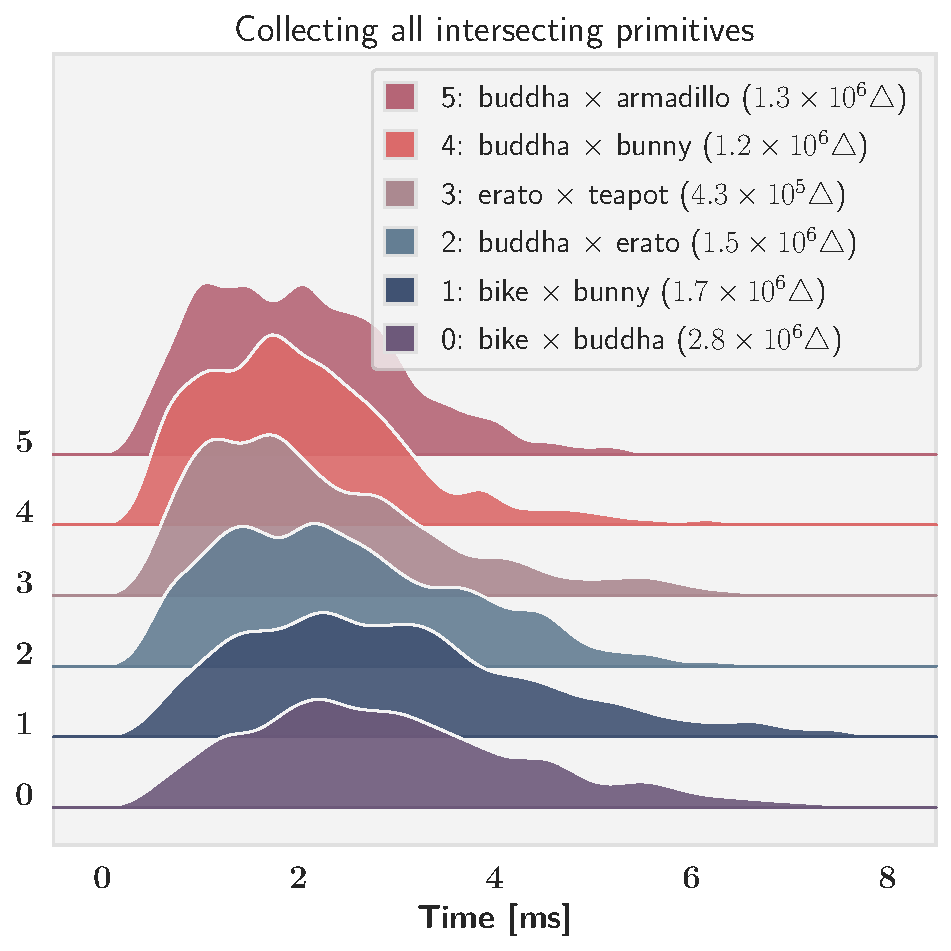
\includegraphics[width=\linewidth]{../figures/intersect-kde.pdf}
\end{minipage}
\begin{minipage}{0.48\linewidth}
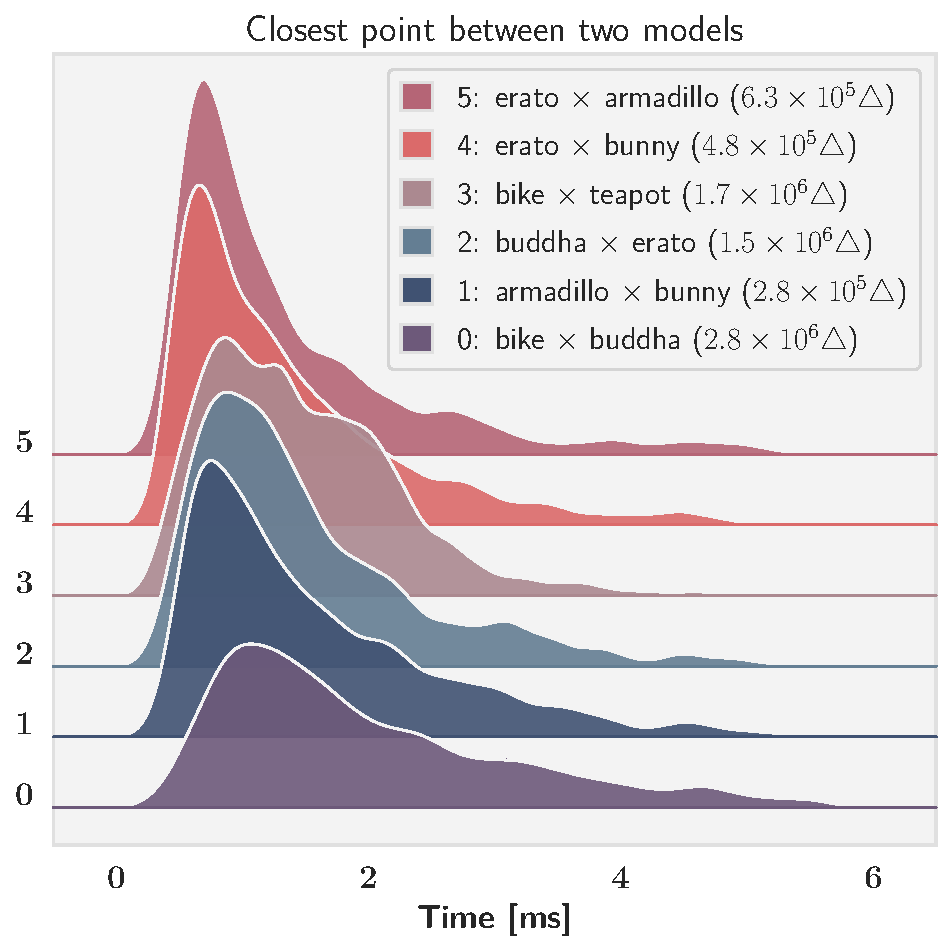
\includegraphics[width=\linewidth]{../figures/closest-kde.pdf}
\end{minipage}
\caption{
Runtime distributions for queries between two models (from Computer Graphics Archive~\cite{McGuire2017Data})
using \texttt{tf::tree} The total number of triangles per query is marked next to $\triangle$.
Each distribution was estimated
on $10{,}000$ samples of relative positions.
\textbf{Left:} Time needed to compute all intersecting
primitives between two meshes. Each sample contained
an intersecting configuration.
\textbf{Right:} Time needed to compute a pair of
closest points between the two models. Each sample
contain a non-intersecting configuration.
}\label{fig:query-dists}
\end{figure*}


\subsection{Contributions}

We introduce \texttt{tf::tree}, a spatial hierarchy designed for high-performance,  
general-purpose geometry queries. The system has been tested in production and  
offers both methodological and implementation contributions to the field.

\paragraph*{Methodological Contributions}
\begin{itemize}
  \item A novel Top-K sorted stack traversal for proximity queries,  
        offering up to $3\times$ speedup over priority-queue-based approaches  
        while maintaining practical cost-efficiency.
  \item An in-depth analysis of selection algorithms for spatial partitioning,  
        with support for pluggable strategies such as \texttt{nth\_element},  
        PDQSelect, Floyd--Rivest, and Alexandrescu's algorithm.
\end{itemize}

\paragraph*{Implementation Contributions}
\begin{itemize}
\item An open-source implementation of
      \texttt{tf::tree}\footnote{\url{https://github.com/xlabmedical/trueform}}  
      that supports search and nearness queries required for interactive geometric  
      modeling; enabling complex processing pipelines such as automatic  
      positioning and boolean operations.
  \item Real time performance in both construction and query time,  
        enabling use in interactive systems. See Figure~\ref{fig:query-dists}
        and Figure~\ref{fig:lib-comparison} for an overview.
\end{itemize}



